\documentclass[sigchi, review, anonymous]{acmart}
\usepackage{booktabs} % For formal tables


% Copyright
%\setcopyright{none}
\setcopyright{acmcopyright}
%\setcopyright{acmlicensed}
%\setcopyright{rightsretained}
%\setcopyright{usgov}
%\setcopyright{usgovmixed}
%\setcopyright{cagov}
%\setcopyright{licensedcagov}
%\setcopyright{cagovmixed}
%\setcopyright{licensedothergov}

% DOI
\acmDOI{10.475/123_4}

% ISBN
\acmISBN{123-4567-24-567/08/06}

%Conference
\acmConference[CHI'19]{ACM CHI conference}{May 2019}{Glasgow, UK}
\acmYear{2019}
\copyrightyear{2019}

\acmPrice{15.00}

% BEGIN ##### LaTeX code added by authors to the preamble #####

\usepackage{soul} %for \hl to highlight
%\usepackage[final,inline,nomargin]{fixme}
\usepackage[draft,inline,nomargin]{fixme}
\newcommand{\hlfixme}[1]{\fxfatal{\hl{#1}}}
\newcommand{\hlfxnote}[1]{\fxnote{\hl{#1}}}

\usepackage{url}      		% llt: nicely formatted URLs
\def\UrlBreaks{\do\/\do-}

\usepackage{array}		%For table column formatting options
\usepackage{dcolumn}    %to align numbers in the table at decimal point
\newcolumntype{d}[1]{D{.}{\cdot}{#1} }

\usepackage{multirow}

\newcommand{\tableheader}[1]{\multicolumn{1}{c}{\textbf{#1}}}

\sloppy
% END ##### LaTeX code added by authors to the preamble #####


\begin{document}

\title{Selective Engagement: A Framework for Limited Use}
%\titlenote{Produces the permission block, and copyright information}
%\subtitle{Extended Abstract}
%\subtitlenote{The full version of the author's guide is available as \texttt{acmart.pdf} document}

%\author{Ben Trovato}
%\authornote{Dr.~Trovato insisted his name be first.}
%\orcid{1234-5678-9012}
%\affiliation{%
%  \institution{Institute for Clarity in Documentation}
%  \streetaddress{P.O. Box 1212}
%  \city{Dublin}
%  \state{Ohio}
%  \postcode{43017-6221}
%}
%\email{trovato@corporation.com}

%\author{G.K.M. Tobin}
%\authornote{The secretary disavows any knowledge of this author's actions.}
%\affiliation{%
%  \institution{Institute for Clarity in Documentation}
%  \streetaddress{P.O. Box 1212}
%  \city{Dublin}
%  \state{Ohio}
%  \postcode{43017-6221}
%}
%\email{webmaster@marysville-ohio.com}

%\author{Lars Th{\o}rv{\"a}ld}
%\authornote{This author is the one who did all the really hard work.}
%\affiliation{%
%  \institution{The Th{\o}rv{\"a}ld Group}
%  \streetaddress{1 Th{\o}rv{\"a}ld Circle}
%  \city{Hekla}
%  \country{Iceland}}
%\email{larst@affiliation.org}

%\author{Valerie B\'eranger}
%\affiliation{%
%  \institution{Inria Paris-Rocquencourt}
%  \city{Rocquencourt}
%  \country{France}
%}
%\author{Aparna Patel}
%\affiliation{%
% \institution{Rajiv Gandhi University}
% \streetaddress{Rono-Hills}
% \city{Doimukh}
% \state{Arunachal Pradesh}
% \country{India}}
%\author{Huifen Chan}
%\affiliation{%
%  \institution{Tsinghua University}
%  \streetaddress{30 Shuangqing Rd}
%  \city{Haidian Qu}
%  \state{Beijing Shi}
%  \country{China}}

%\author{Charles Palmer}
%\affiliation{%
%  \institution{Palmer Research Laboratories}
%  \streetaddress{8600 Datapoint Drive}
%  \city{San Antonio}
%  \state{Texas}
%  \postcode{78229}}
%\email{cpalmer@prl.com}

%\author{John Smith}
%\affiliation{\institution{The Th{\o}rv{\"a}ld Group}}
%\email{jsmith@affiliation.org}

%\author{Julius P.~Kumquat}
%\affiliation{\institution{The Kumquat Consortium}}
%\email{jpkumquat@consortium.net}

% The default list of authors is too long for headers.
\renewcommand{\shortauthors}{S. Patil et al.}


% !TEX root=nonusecomments.tex
\begin{abstract}
Owing to its exponential rise in popularity and adoption, social media usage has received extensive research attention in the past decade. Recently, however, researchers have started to recognize the need to pay attention to negative aspects and non-use of social media in order to uncover barriers and surface shortcomings of these systems. We contribute to these efforts by analyzing user-generated comments on posts related to Facebook on blogs with a tech savvy readership. We found that nearly half of total 3000 randomly selected reader comments indicated negative sentiment and described implied or explicit non-adoption. Our findings highlight the importance of utilizing user generated content as a tool for large scale user feedback. Moreover, we highlight that expert perspectives can aid in early surfacing of problematic aspects.
\end{abstract}
%Further qualitative coding revealed privacy concerns and user experience as key factors.

%
% The code below should be generated by the tool at
% http://dl.acm.org/ccs.cfm
% Please copy and paste the code instead of the example below.
%
\begin{CCSXML}
<ccs2012>
 <concept>
  <concept_id>10010520.10010553.10010562</concept_id>
  <concept_desc>Computer systems organization~Embedded systems</concept_desc>
  <concept_significance>500</concept_significance>
 </concept>
 <concept>
  <concept_id>10010520.10010575.10010755</concept_id>
  <concept_desc>Computer systems organization~Redundancy</concept_desc>
  <concept_significance>300</concept_significance>
 </concept>
 <concept>
  <concept_id>10010520.10010553.10010554</concept_id>
  <concept_desc>Computer systems organization~Robotics</concept_desc>
  <concept_significance>100</concept_significance>
 </concept>
 <concept>
  <concept_id>10003033.10003083.10003095</concept_id>
  <concept_desc>Networks~Network reliability</concept_desc>
  <concept_significance>100</concept_significance>
 </concept>
</ccs2012>
\end{CCSXML}

\ccsdesc[500]{Computer systems organization~Embedded systems}
\ccsdesc[300]{Computer systems organization~Redundancy}
\ccsdesc{Computer systems organization~Robotics}
\ccsdesc[100]{Networks~Network reliability}


\keywords{ACM proceedings, \LaTeX, text tagging}

%\begin{teaserfigure}
%  \includegraphics[width=\textwidth]{sampleteaser}
%  \caption{This is a teaser}
%  \label{fig:teaser}
%\end{teaserfigure}

\maketitle

% !TEX root=nonusecomments.tex
\section{Introduction}
\label{sec:introduction}
%Since their inception in early 2000s, social network sites and social media have transformed everyday interactive practices. Today, the most popular of these sites, Facebook, claims more than 2 billion global active users. As of 2016, 79\% of Internet users (68\% of all U.S. adults) are estimated to use Facebook~\cite{greenwood2016social}. Such explosive growth and popularity has resulted in a great deal of research attention toward the use and positive impacts of social media in general, and Facebook in particular. For instance, it has been shown that the use of Facebook can be associated with a number of benefits, such as enhancing social connectednedness, increasing social capital, and boosting self esteem~\cite{koroleva2011its,ellison2007benefits}.

%However, more recent research indicates that increased use of social media may also lead to a number of negative effects, including addiction, feelings of jealousy, depression, decreased well-being, invasion of privacy, reduced work productivity, cyberbullying, etc. As a consequence, people have reported efforts to reduce their use of social media via tactics such as taking a ``vacation'' from Facebook or deleting their accounts. For instance, recent Facebook scandal that exposed large-scale harvesting of its user data by the British firm Cambridge Analytica resulted in the trending hashtag \#deleteFacebook.

%In the past few years, researchers have recognized the need to investigate such ``non-use''~\cite{baumer2014refusing}. However, barring a couple of notable exceptions~\cite{baumer2013limiting,lampe2013users}, research on non-adoption, non-use, and abandonment of Facebook has received disproportionately little research attention. Moreover, as Facebook functionality and policies change and people's knowledge and experience regarding Facebook evolve, initial findings regarding non-use may need to be updated correspondingly. To this end, we formulated the following research question:





Emergence of technology and continuous integration of internet based services in everyday life has introduced the era of ``Big Data''~\cite{lohr2012age}. While such advancement has flourished user experience in many aspects, it has engendered other user related issues as well, such as privacy concern~\cite{shin2010effects}, data breach etc. Such issues are important to take into account while designing secure and reliable system. Owing to privacy issues users can reduce and even abandon further engagement with the system~\cite{madden2012privacy} which makes this a burning question for system developers, UX designers, and advertisers alike. The proliferation of social media sites and corresponding user interaction thus invoke issues that might lead to Negative Sentiment \emph{(NS)}, and lack of usage (\emph{Non-use}). Factors that contribute to \emph{NS \& Non-use} can threaten the sustainability and success of these systems. Therefore, a comprehensive understanding of non-usage from technical and sentimental point of view is required for building a successful ecosystem of user base.

%However, prior research on those who reduce the usage, refrain from using or totally abandon a system has not been exhaustive.  In this study, therefore, we want to unveil individual, social, and technical factors that underlie non-adoption, abandonment, and non-usage of a system. In particular, we want to uncover the barriers of privacy and security concerns, socio-economic and individual issues that results in reduced engagement. In this paper, we will investigate what factors lead to resisting, dropping out or lurking. Some of the factors that often lead to such behaviour are often- taking 'vacation' from social media, minimize their wasting time, privacy concerns, disliking a particular feature etc.

Although prior research focused on adoption of technologies and various benefits of usage~\cite{joinson2008looking}, little has been studied on those who possess \emph{NS} about and eventually reduce the usage, refrain from using or totally abandon a system~\cite{wyatt2003non}. Few studies attempted to address this issue by explicit questioning of regular users~\cite{baumer2013limiting, nonnecke2001lurkers}. To fill in this gap we wanted to investigate this scarcely studied user population~\cite{baumer2014refusing} and user generated content from a tech-savvy user environment. From a wide range of choices we picked Slashdot\footnote{\url{https://slashdot.org/}} (``News for Nerds. Stuff that Matter'', as they say) and Schneier on Security\footnote{\url{https://www.schneier.com/}}. Slashdot is a technology-related news website, the summaries of stories and links to news articles are submitted by its own readers, and each story becomes the topic of a threaded discussion among users. Bruce Schneier's blog is a collection of article/stories, hacks and latest news on Information Security where privacy experts discuss the state-of-art privacy and security concern on latest technology. It is safe to assume these users are technology geeks and we get spontaneous unprompted content from their comments. The motivation behind using these two different sources of data is to get better insight about Facebook haters \& non-users and compare the findings with an assumption that they will agree or disagree to some extent. We randomly collected 2000 comments that belong to the ``Facebook'' category from Slashdot and 1000 comments from Schneier's blog, and analyzed them with an aim to answer the following research question:


\begin{quote}
    \textit{RQ1: Do expert users possess negative sentiment towards technology and are actually rejecting it (Facebook in our case)?} (By rejecting we mean reduced or passive usage, dropping out, and resistance towards Facebook.)

\end{quote}
% To collect and analyze people's view and opinion regarding \emph{'Non-use'} we consulted various social media forum based sites and picked \textit{Slasdhot}. Slashdot is a technology-related news website, the summaries of stories and links to news articles are submitted by its own readers, and each story becomes the topic of a threaded discussion among users. Earlier studies though focused on non-usage of Facebook, didn't focus on the particular technology friendly group of users who interact heavily online. The active discussion in \textit{Slasdhot} not only provided a means to unveil the reasons behind the usage to non-usage transition of an individual in social media but also helped us analyze of different contexts on which the comments were made. 

 In general, we used qualitative binary coding to determine the comments related to Facebook Negative Sentiment \emph{(NS)} and \emph{Non-use}. Two coders individually coded the randomly selected scraped comments of Slashdot and Schneier's blog. The method of randomization was used to avoid any form of biases which can occur to collect the data during a particular time-period. Later, on the comments coded as \emph{NS} by either one of the coders, we did extensive qualitative coding  to probe more on the reasons of Facebook \emph{NS}. We classified comments into \emph{explicit Non-use} \& \emph{implicit NS} and performed thematic coding to investigate what reasons (privacy and security concerns, socio-economic and individual issues etc.) lead to resisting, dropping out or lurking. In particular the focus was on individual, social, and technical factors that underlie the \emph{NS} and eventual non-adoption, abandonment, and non-usage of a system. 
 
 \begin{quote}
    \textit{RQ2: What factors underlie Facebook \textit{NS}, non-usage and non-adoption by techies?}

\end{quote}

We presented the extent to which expert users are expressing their concern towards Facebook in two different blogosphere and how their opinions vary. This is extremely important since the underlying factors might shape the way the future systems are designed by engendering future research in the concern areas. We observed that \textit{privacy \& security concerns}, aspects related to Facebook (\textit{user experience}), and \textit{personal preference} were 3 of the 10 key factors responsible for \emph{NS} and \emph{Non-use}. In fine, the main contribution of this paper is an extension of methods used to gain insight regarding user discontent, \textit{Non-use} and non-adoption. Further, we focus on the tech-proficient population who are often an early adopters of technology. \emph{NS} of such individuals can illuminate important design or operational shortcomings, especially for privacy and security matters that often require nuanced technical understanding. Moreover, we utilize naturalistic user-generated content to confirm and refine previous research on factors that underlie various forms of \emph{NS} and behaviors pertaining to \emph{Non-use}. To this end our contribution is unique since comments acquired from such blogs/forums are in their intended social context in realistic settings instead of interview or lab environments, where study of \emph{NS, Non-use} has been conducted previously.


In the rest of the paper, we first discuss all relevant prior work followed by presentation of our methods extensively and showing why thematic qualitative coding made our results effective. Then we illustrate our findings based on empirical study and further discuss the findings in detail. Thereafter, we argue on the practical implications for our findings in real world. We also discuss a few challenges faced during this work, limitations, and potential future works in the end. Then we conclude our study by summarizing the findings. 

% !TEX root=nonuseinterviews.tex
\section{Related Work}
\label{sec:relatedwork}
The Internet is shaping how we communicate with each other~\cite{wellman2003social} and social media paved the road of communication~\cite{bijker2012social}. Facebook is the largest social networking website and despite criticisms, its usage continues to grow~\cite{joinson2008looking}. However, we notice users concerns regarding various features of Facebook, including its data usage policy, often moving to other social media platforms?, privacy concerns regarding posted content, advertisements, and others. These concerns lead to reduced posting, increased lurking, self-censorship, and even abandoning the platform all together~\cite{wyatt2003non,karppi2011digital,gillette2015facebook}. The creation of a Facebook quit day, where people commit to quit Facebook and never return is an example of these practices\footnote{\url{http://www.quitfacebookday.com}}. 

Technological non-use has been a matter of concern for Human Computer Interaction (HCI) scholars as it not only focuses on the design changes, it also focuses on the user experience as a whole which is a critical predictor of improved security adoption and use~\cite{baumer2015importance}. Though much work is being done on usage of social media, there are essential literature gaps in understanding the dissatisfaction in consumer base, specifically of Facebook, through qualitative research. This related work section aims to provide a comprehensive analysis of the user cited reasons through different works expressing concerns on the usage of social media, especially Facebook.

\subsection{Lurkers and Non-Usage}
Lurking is defined and interpreted differently by various researchers~\cite{crawford2009following,schultz2004lurkers} and while discussing non-use it is very important not only to discuss usage versus non-usage but also to focus on users curtailing their usage in different levels. For our study, we focus on lurkers who have curtailed their usage specifically on Facebook. We also address users who have reduced their usage and abandoned the platform entirely.

Previous studies into Facebook lurking, reduced usage, and non-usage found that there are varied contributors that lead to limiting the use of Facebook to a minimal level, deactivation of accounts, and deletion of accounts. While different factors drive these changes in the user base, one common factor which was present among the users in this study were concerns that they have regarding their privacy on Facebook~\cite{baumer2013limiting}. Nonnecke et al.~\cite{nonnecke2001lurkers}, Preece et al.~\cite{preece2004top}, and Birnholtz~\cite{birnholtz2010adopt} explored the reasons behind lurkers studying several groups over Internet through interviews, however Facebook is a larger community and warrants separate study since Facebook abandonment can arise from specific features including advertisements, moderated news feed, email notifications, etc. These studies, however, while similar in subject matter and methodology differ in the approach as well as the granularity of non-usage. 

\subsection{Privacy Concerns}
Users have become increasingly aware of privacy concerns~\cite{hargittai2010facebook}, specifically in the post-Snowden era~\cite{rainie2015americans}, and more users have switched their account to Friends Only or Custom Settings compared to the first few years of Facebook~\cite{fuchs2012political,madden2012privacy}. This shift might also be explained by a lack of granular privacy settings earlier in Facebook's history as opposed to newer privacy controls. More than half of social media users (58\%) restrict access to their profiles by customizing the privacy settings, especially women~\cite{madden2012privacy}. We noted similar results as discussed in the Section~\ref{sec:findings}.

Participants in our study also mentioned that with age the amount of disclosure reduced, similar to Nosko et al.'s work~\cite{nosko2010all}. Lampe et al. argue that privacy plays a vital role in users not joining Facebook~\cite{lampe2013users} and even leading to commit virtual (social media) suicide by leaving the platform~\cite{stieger2013commits}. Perceived privacy and security, though might be different from the actual practices preached, plays a vital role in user interaction over social media~\cite{jung2016imagined,shin2010effects,debatin2009facebook,liu2011analyzing}. These concerns are enhanced for romantic partners whose Facebook experience is made more difficult due to  omnipresence of data and the ability to track a partner's posts~\cite{gershon2011friend,madden2006online,zhao2012s}. Stories from families and friends about privacy and security concerns also play an influential role in reduction of usage by Facebook users~\cite{rader2012stories}. 

Privacy and security concerns vary among different individuals indicating privacy inequalities~\cite{litt2013understanding,kang2015my} and can have important implications in design of a system~\cite{dupree2016privacy}. What is practised and preached in privacy and security concerns vary greatly ~\cite{phelan2016s} and it becomes difficult for researchers and developers to understand the details with such granularity and specificity. As a result, a binary classification as use vs.\ non-use is unable to fully characterize non-use practices of individuals. With our study, we aim at clustering various concerns leading to different or similar attitudes and behaviors of social media users and generate a typology of non-use.

\subsection{Monitoring Old Habits}
Bauer et al., found that users desired to have the ability to go through old posts as well as modify or enhance their privacy settings ~\cite{bauer2013post}. This, often referred to as monitoring, indicates that users want to represent themselves in a way that their past posts do not justify. Self-representation is extremely important for social media users~\cite{dimicco2007identity,zhao2008identity}, thus monitoring their virtual image is of high importance as well. Our analysis, as explained in Section~\ref{sec:findings} indicates similar patterns among the users where they have expressed interest in a better way to monitor their posts and sometimes delete it.

\subsection{Audience and Other Social Media}
The audience of social media, especially Facebook, is transitioning from the younger generation to older individuals which contributes to the non-usage of Facebook. The inter generational social media usage difference is increasingly blurring~\cite{bucur1999older}. Bauer et al. suggests that users may be leaving sites like Facebook in favor of newer platforms like Snapchat. On Snapchat, a photo stays in the story only for 24 hours, and the user is notified if another user takes a screen shot of the photo~\cite{bauer2013post}. We noticed similar reactions from some of our participants as well, thus, indicating some users do not like the permanency of the posts made on Facebook. 
%However our results signify that this depends on several factors. A participant expressed using Facebook as personal media storage, indicating positive implication of such a feature.

\subsection{Abusive Posts}
Mental and physical health is often considered to be a primary source of concern. Social media, though purportedly just a medium to connect individuals, has often been noted to affect users negatively, sometimes due to usage time and sometimes due to abusive content~\cite{newyorktimes2017}. Our research showed that users, including supporters of free speech, often expressed dissatisfaction regarding abusive posts, especially regarding religious or political sentiments. Adults are however less affected as compared to teens~\cite{lenhart2011teens,rainie2012tone} by such posts, but the abusive nature of the content not only contributes to bullying over the Internet, but also leads to the discontinuation of the use of such sites.

\subsection{Social Influence}
Non-Use though a personal choice can be influenced positively or negatively by various other social and behavioral factors. Baumer et al. used a survey to study how several factors including, fear of missing out, reaction of one's social media audience impact one's perspective of not being able to leave a system~\cite{baumer2015missing}. Though survey techniques  provide an overall archival reasons for non-usage of social media platforms it does not provide the detailed analysis of what prevents one from completely abandoning such platforms. As mentioned by Baumer et. al's paper, every method including surveys to machine learning including qualitative and quantitative techniques have unique approaches to a similar problem providing more and detailed analysis of a problem~\cite{baumer2017comparing}.

Baumer et. al's other studies on details of deactivation of Facebook and reduction of usage of social media provide a mixed-methods view based on surveys to interviews. However, it demarcates the usage between group communication and whether people chose to deactivate or not~\cite{baumer2017subjects}. One's usage of social media is not binary (use and non-use) or ternary (use, limited use, and non-use). Instead, non-use may cover a wide spectrum of practices involving various levels of engagement on social media.
%Squirell in this article mentions how trolls are leading to hate speeches and even frog memes are one of the most rated hate symbols ~\cite{squirrell_2017}. 

\subsection{Miscellaneous Reasons for Lurking}
Though studies on non-usage have not been limited to Facebook, but have also covered other social media platforms, such as Twitter~\cite{schoenebeck2014giving}, varying levels of (non-)usage is still understudied. Ames et al. identified the negative effect of multitasking as one of the primary reasons for lurking on social media~\cite{ames2013managing}. Whereas, Portwood argued that the fear of misinterpretation is one of the key reasons for reducing usage on Facebook~\cite{portwood2013media}. There are arguments about the digital divide and how it prevents one from communicating similarly to a privileged individual, contributing to the avoidance of social media all together~\cite{van2005deepening,warschauer2004technology}. Hargittai explores more on the social divide by mentioning that people with more technical expertise are likely to use social media~\cite{hargittai2007whose}. Ryan and Xenos instead try to analyze the characteristic traits of individuals who use Facebook, thus indicating the negative traits by exploring the Big 5 characteristics~\cite{ryan2011uses}. Verdegem and Verhoest grouped all the traits for non-use together, mentioning inaccessibility, lack of skills, and negative perception of the technologies to be the key reasons to reduce usage~\cite{verdegem2009profiling}. Design issues have also been considered in making users cease usage of Web site~\cite{pierce2012undesigning,satchell2009beyond}. All these reasons though effective is highly scattered across various facets of social media. We apply our findings to make design recommendations for Facebook to improve its user experience (see Section~\ref{sec:implications}).

% !TEX root=foo.tex
\section{Method}
\label{sec:method}
% This study involved collection of data from a popular technology news site, Slashdot. We collected 1000 comments related to Facebook and use. we then implemented a multi-level human coding to probe into why Facebook usage is reducing everyday. We chose Slashdot to particularly focus on the techies. Often the techies are removed from data collection to obtain an unbiased sample. However the people concerned about their privacy and security online are increasing everyday and they are playing a vital role in altering the user base of social media websites like- Facebook. We also applied topic modelling and sentimental analysis to avoid the limtiation of only human coding.

In this section, we discuss how we performed two level of codings followed by the topic modeling, sentiment analysis, and wordcloud generation methods:

\subsection{Data Collection}
We compiled a new corpus of articles and related comments from a technology news site: Slashdot. This site was chosen for several reasons: Slashdot was voted one of Newsweek's favorite technology web sites and rated one of Yahoo's top 100 web sites as "Best Geek Hangout".\footnote{\url{http://digitalenterprise.org/cases/slashdot.html}} So we can infer that posters and commenters of Slashdot are tech-savvy users and have better insight of the pros and cons of state of the art technology. Therefore, their reviews are critical in understanding the existing \emph{Non-use} of social media (Facebook in our case) and related sentiments. Also, we were looking for a discussion based blog or forum from where we can get unprompted naturalistic responses. Comments on Slashdot are moderated by users of the site, each comment has a score between -1 to +5 which ensures high quality contribution and discouraging spams or vandalism. Each moderator in Slashdot is able to modify the score of a given comment by +1 or -1. Furthermore, each comment is classified in several categories: for good comments, the classes are: Interesting, Insightful, Informative, and Funny. For bad comments, the classes are: Flamebait, Troll, Off-Topic, and Redundant. Posts are associated with topic tags, such as political, facebook, social media, science etc. 

Slashdot comments are displayed in a threaded tree type discussion conversation. Commenters can reply in a given thread and subsequent replies for that comment appear in hierarchical order. We scraped the whole history of posts and associated comments since the inception of Facebook (2004) till date. We used Python \textit{BeautifulSoup} and \textit{Scrapy} for crawling and the data was saved into MongoDB in JSON format. For our purpose of analysis, we only considered the posts which have a topic tag "Facebook". The comments that we collected for analysis have been filtered based on the following factors: 
\begin{itemize}
    \item contains the term "Facebook", "FB" or "Social Media" in body or title for relevance.
    \item minimum 100 characters in length for better understanding of context.
    \item minimum score of +2 to ensure high quality comments.
\end{itemize}
\subsection{Binary Coding}
A random sample of 1000 comments that satisfy the aforementioned criteria were collected from the whole dataset. Later, they were manually coded by two independent coders (first and second author) to check if they belong to either one of the class \textit{Non-use} or \textit{not related to Non-use}. If a particular comment reflected harsh criticism of Facebook, inactive or passive usage, reduced usage or complete abandonment: the coders classified that comment as \emph{Non-use}. Other comments which discussed all other different topics related to Facebook were marked as \textit{not related to Non-use}. One typical such example of \emph{Non-use} comment is:
\begin{quote}
    \textit{The future does not look so bright for facebook as they will probably suffer the same fate as usenet. Sounds like a positive outcome to me. The world would be better off without the cancer that is facebook.}

\end{quote}

To make sure both the coders are on same wavelength, we checked the agreement after coding 500 comments. It turned out we achieved 78.3\% agreement with the Cohen's $\kappa$=0.56. Later, we checked a subset of 20 of the disagreements and had a discussion to resolve the discrepancies and come to an agreement. Then we individually re-examined all other disagreement cases and checked if we wanted to keep or change our original classification. It was discovered that the raters encountered one major point where both of them disagreed mostly: initially all the comments that explicitly stated or expressed some form of \emph{Non-use}, such as "deleted my account...", "not using for long...", "I hate Facebook..." etc. were marked as \textit{Non-use} only by one rater while the other rater also insisted to incorporate comments related to harsh criticism or sarcasm of Facebook. This was reasonable since in such cases users might not explicitly mention about the \textit{Non-use} but their aversion towards Facebook is visible which might lead them or encourage other users to \textit{Non-use}.  After the discussion on the remaining disagreements, the agreement rate was 92.8\% with the Cohen's $\kappa$=0.856. After coding all 1000 comments, the overall agreement rate was 93.6\% with the Cohen's $\kappa$=0.872. Table~\ref{tab:table1} summarizes the categories assigned by the raters. Only 64 (6.4\%) times the raters disagreed. Since we got a high agreement score, we picked 516 (452+21+43) comments which were marked as \textit{Non-use} by one or both the raters for second level thematic coding.


\newcommand{\head}[1]{\textnormal{\textbf{#1}}}

\begin{table}[!ht]
% let LaTeX figure out optimal amount of intercolumn whitespace:
\setlength\tabcolsep{0pt} 

\begin{tabular*}{\columnwidth}{@{\extracolsep{\fill}}c*{3}{T{1.8}}cT{1.8}}  
\toprule
\head{First/Second Rater} & \head{NU} & \head{NRNU}\\
\midrule
\textbf{NU}              & 452     & 21 \\                    
   \textbf{NRNU} & 43      & 484 \\
  \hline
\bottomrule 
\end{tabular*}
\caption{Categories assigned by two independent raters on 1000 comments. (NU = Non-use, NRNU = Not Related to Non-Use)}
    \label{tab:table1}
\end{table}
\subsection{Thematic Coding}
After coding 516 comments in \emph{Non-use} category as discussed above, we wanted to expand more on finding the reasons of \emph{Non-use} by the Facebook users. We performed a second level thematic coding by implementing the coding categories of Das and Patil's paper~\cite{das2017resistance}. We could not extrapolate all the categories generated from that paper due to nature of differences in our data. We observed a subset of 7 coding themes which encompassed all of our comments and the remaining did not appear. Another exclusive category that appeared but we did not report was \textit{Modified Behavior}, because comments belonging to this category reflected change in user interaction with Facebook but it was more of an effect than a cause. One such comment is:

\begin{quote}
    \textit{I left facebook a few months ago and specifically requested deletion, not deactivation. There was a 14 day waiting period, during which time I could log back into my account and reset the clock, but supposedly at the end of those 14 days my account was gone for good. From what I can tell [facebook.com] they still allow you to do this: "If you don't think you'll use facebook again, you can request to have your account permanently deleted. Please keep in mind that you won't be able to reactivate your account or retrieve anything you've added."}

\end{quote}

However, we keep those comments for study as they were marked as \textit{Non-use} in the first place. But for the purpose of simplicity of explanation and NLP analysis, we will count it as the eighth theme. Table~\ref{table:coding category} describes these 7 themes implemented by the authors of this paper, number of comments belonging to that theme and one example comment. The theme titles are self-explanatory yet we give some keywords or topic words (second column) per theme which will help elucidate the coding criteria.    

% . From our comments, we coould classify some of the comments signifying having a Facebook account or not, however we cannot classify accordingly for all the categories. Thus, we chose a subset of the coding categories which consisted on 7 coding categories were generated by exploring the qualtitaitve study of interviews. Table~\ref{table:coding category} describes the coding categories implemented by the authors of this paper and a few examples as discussed later.

The two coders who coded the binary coding, coded a first set of 100 comments of the 516 \emph{Non-use} comments.  Initially we only allowed a single code per comment for the first set of coding. We noted the inter-coder reliability score was 70.4\% with the Cohen's $\kappa$=0.637. The rating was fairly good, however we discussed about the coding scheme and noted that due to the nature of some of the comments we could not classify one comment only under a single theme. After discussing further, we decided on coding a single comment for multiple themes. For example, the following quote by one of the commenters not only shows that they are not using Facebook due to Facebook's feature of tagging users (indicating Facebook functionality influence as user dissatisfaction) but also indicates about the audience activity of tagging users. Both the users coded this comment under \textit{Audience} as well as \textit{Facebook Functionality}.
\begin{quote}
\textit{I don't use Facebook. That doesn't stop my friends from tagging my face when I'm in one of their photos which they post on Facebook.}
\end{quote}
After the thematic coding of a total of 100 comments, we found the inter-coder reliability score of 89.8\% with the Cohen's $\kappa$=0.87. With this inter-coder reliability score, we coded the rest of the comments and found that the inter-coder reliability score after coding all the 516 was 97.3\% with the Cohen's $\kappa$=0.966. The thorough coding not only enabled the coders to analyze the non-usage aspect of Facebook users but also indicated the specific reasons on why the users are behaving in a certain way leading to Facebook rejection of some form. 

\subsection{Wordcloud and Topic Modeling}
We performed NLP based analysis to get a sense of the innate sentiment of the commenters as well as the reasons for their deliberate \textit{Non-use}. Wordclouds have been particularly useful to get a top level idea and has been widely used for text mining \cite{younis2015sentiment}. We picked the 516 comments those were marked as \textit{Non-use} and built wordcloud using Python \textit{wordcloud} package. The initial wordcloud had irrelevant terms which are not informative, such as "facebook", "would', "say" etc. Therefore, we created a custom list of stopwords ourselves besides the Python package \textit{nltk} provided list of stopwords. To get better insight, we created bigram and trigram wordcloud on the same dataset using \textit{tm} library of R. Data was preprocessed and cleaned using process described in ~\cite{wang2013gender}. While we removed the stopwords for unigram and bigram wordclouds, it was not done for trigrams as we wanted phrases like "i hate facebook", "i don't care" etc. The results are dicussed in the following section.

Besides wordclouds we performed Latent Dirichlet Allocation (LDA) topic modeling \cite{blei2003latent} to surface the hidden topics (sentiment words, non-use related terms) from the comments. LDA is a statistical method that assumes a corpus is a mixture of topics and a topic is mixture of words ~\cite{suresh2015autodetection,wang2013gender}. We used the python library \textit{Gensim} and trained the model on 516 \textit{Non-use} comments after cleaning the data (removing punctuation, proper names, tokenizing and lemmatizing). The number of topics were chosen as $K=8$ for two reasons: we got 8 factors from the thematic coding and the topics started repeating after this threshold hence becoming less interpretable. We made sure to eliminate words that only appeared a few times and generic words that appeared several times. This helped improving the information gain and finding better topics by fast convergence. Each topic is associated with weighted words under that topic and the high weight represent most depictive word of that particular topic. 

To confirm our results of LDA topics, we implemented another popular topic modeling approach called Non-negative Matrix Factorization (NMF) because it is better at compact semantic representation of documents in small data setting ~\cite{choo2013utopian}. Using tf-idf ("term frequency-inverse document frequency") from \textit{scikit-learn}, we converted each document in corpus to vectors. One important thing to note is, we had to set minimum and maximum document arguments to get rid of too generic or too unlikely words. The number of topics were chosen as 8 for the similar reasons mentioned above.

\subsection{Sentiment Analysis}

To understand the polarity of sentiments of users, we performed sentiment analysis on the comments. We used VADER (Valence Aware Dictionary and Sentiment Reasoner), a lexicon and rule-based sentiment analysis tool that is specifically engineered to extract sentiments expressed in social media. It incorporates qualitative and quantitative methods and performs as well as other standard benchmarks for sentiment analysis (e.g., LIWC, ANEW, the General Inquirer, and machine
learning based techniques) ~\cite{hutto2014vader}. We performed overall and theme wise (8 influential factors mentioned above) sentiment analysis using \textit{vaderSentiment} package in Python and reported the compound sentiment score and associated sentiment (positive or negative). One important adjustment that we made while doing this analysis was: we filtered out non sentiment related terms and picked the opinion terms instead. This technique was proposed by Pang and Lee ~\cite{pang2004sentimental} to remove objective sentences by extracting subjective ones. Often times in lexicon based sentiment analysis in a review or comment (especially long ones), it is observed that the non-sentiment related sentences affect the overall sentiment polarity of the review. To overcome this, we adopted a simple approach to filter the opinion sentences from the corpus. We took advantage of the list of positive and negative words compiled by Hu and Liu~\cite{hu2004mining} (2005 positive and 4783 negative words). From each comment, the sentences that contain at least one sentiment word from above list (positive or negative) were retained. We call them the \emph{opinion sentences}. The remaining analysis was routinely performed using VADER tool, and  the categorization of scoring and interpretation of results are given in the following section.

% In order to get contextual polarity from the comments and compare our results with findings obtained above, we also trained a logistic regression model. This is a simple linear model and is widely used for sentiment classification. To train the model, we used the data provided by Kaggle\footnote{\url{https://inclass.kaggle.com/c/si650winter11}}. Every training data is a sentence extracted from social media (blogs). The training data contains 7086 sentences, already labeled with 1 (positive sentiment) or 0 (negative sentiment). With help of Python \textit{scikit-learn}, we converted the corpus into matrix of tokens (after all preprocessing). Then we performed logistic regression using 85\% of input data for training and remaining 15\% for validation (for accuracy estimation). The trained model was applied on our theme wise comment set for sentiment classification and the findings are discussed in Findings section.
 





% !TEX root=foo.tex
\section{Findings}
\label{sec:findings}

\subsection{Qualitative Coding}

As discussed in the previous section, we filtered 516 comments based on the initial binary coding which account for more than half (51.6\%) of the dataset of 1000 comments. Later, we performed second level thematic coding based on 8 themes (although we report 7, the clarification on eighth one is given in Methods section) mentioned previously to see what is the underlying factor for either social media \textit{Non-use} or user dissatisfaction. The findings are summarized in Table~\ref{table:coding category}.


\begin{table*}[t!]

\centering
\begin{tabular}{p{0.20\linewidth}|p{0.2\linewidth}|p{0.1\linewidth}|p{0.4\linewidth}}
\hline
{Theme} & {Example Topic} & {\# Comments} & {Example Comment}  \\
\hline
Facebook Functionality  & advertisement, news feed, messenger, tagging   & 245(222) & \textit{"After all, Facebook users have NO CHOICE but to use Facebook and allow them to force you to watch ads. Really, you have no choice, none at all. Suck it up and get used to it."}\\\hline

Privacy and Security & selling data, stalking, apps accessing mobile data & 168(158) &\textit{"Facebook is essentially saying you don't HAVE to enter into an agreement with them in order for them to keep track of you."}\\\hline

Personal Preferences & waste of time, do not like using Facebook, do not care & 96(85) &\textit{"who cares? I DO NOT GIVE A DAMN, I don't use Facebook or linkedin, and my computer blocks resolving those domains."}\\\hline

Negative Perceptions of Facebook & creepy, blocked Facebook, hate words & 76(64) &\textit{"Seriously, I've distrusted Facebook from the very start, and never will trust it. Given that Zuckerberg is on record as saying that anyone who trusts him is a fool, I'm going to work accordingly. I've got better things to do with my life then spend it tethered to bullshit."}\\\hline

Audience & sharing data with friends, audience changing, impression management & 67(63) &\textit{"The proper form that the apology should have taken is this, "I am sorry that anyone was offended because someone added me to a Facebook Group that included tasteless comments, comments that may constitute illegal threats of violence, made by someone else. I do not condone such language."}\\\hline

Influence of External Factors & forced to use, job, politics & 58(45) &\textit{"About a year ago, keeping up with FB started to seem like a bit of a job, ain't nobody paying me to do it, and it has seldom if ever proved all that helpful or useful in ways that couldn't be accomplished via other, less intrusive, less annoying ways"}\\\hline

Non-Facebook Media Use & migrating to other social media, preferring other social media, telephone & 27(21) &\textit{"My teenage daughters, and all their friends, live and breathe SnapChat. Not one of them is on Facebook. This could change, but I don't anticipate any of them switching."}\\\hline
\hline
\end{tabular}
\caption{Themes from second level thematic coding, example topic, number of comments, and one representative example. Within parentheses is the number of comments where both rater agreed for that theme and outside where either one agreed.}
    \label{table:coding category}
\end{table*}


The distribution of the comments falling into each theme is depicted in Figure~\ref{fig:figure1}. We have shown, for each theme, the number of comments that fell into that theme. It is obvious from the graph that in all cases the raters disagreed to some extent. The percentages shown as label on blue bars does not sum to 100 since one comment could be associated with multiple themes therefore those comments are counted multiple times.

\begin{figure}
  \centering
  \includegraphics[width=1.0\columnwidth]{figures/fig7.jpg}
  \caption{Distribution of 516 \emph{Non-use} comments into themes.}~\label{fig:figure1}
\end{figure}

\subsection{Natural Language Processing}

\subsubsection{Wordcloud}
We performed multiple NLP based analysis on our dataset to gain deeper understanding. The initial unigram wordcloud that was made on overall 516 \textit{Non-use} related comments (regardless of theme) is shown in Figure~\ref{fig:figure2}(a). Drawing a bigram (Figure~\ref{fig:figure2}(b)) and trigram (Figure~\ref{fig:figure2}(c)) helped us surface further innate emotions and reasoning of Facebook haters.


% \begin{figure*}[t]
% \centering
% \subfloat[Unigram wordcloud ]{
%   \includegraphics[width=60mm, height=4cm]{figures/fig2.png}
% }\hfill
% \subfloat[Bigram wordcloud]{
%   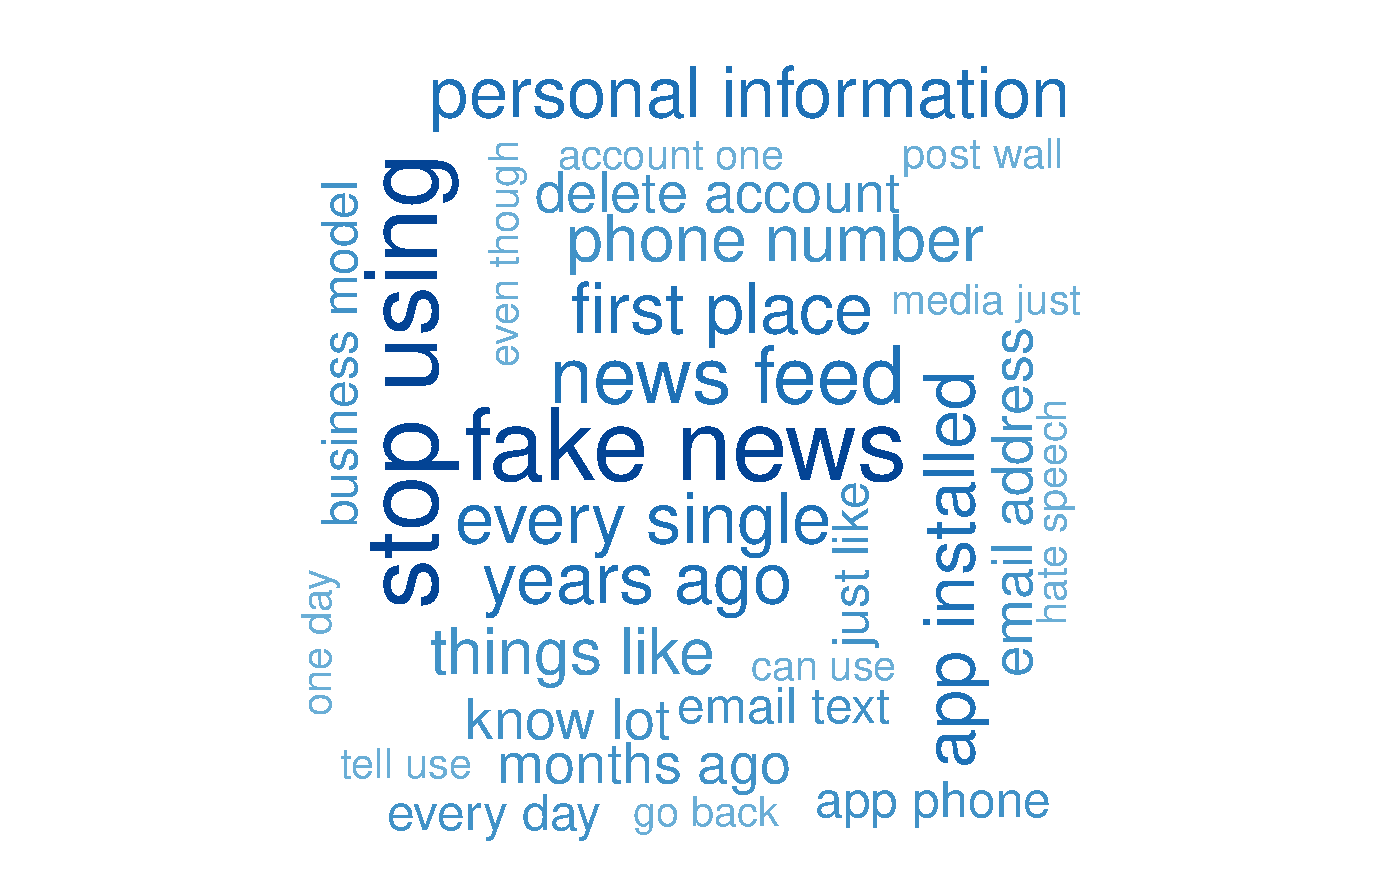
\includegraphics[width=90mm]{figures/fig3.eps}
% }\hfill

% \subfloat[Trigram wordcloud]{
%   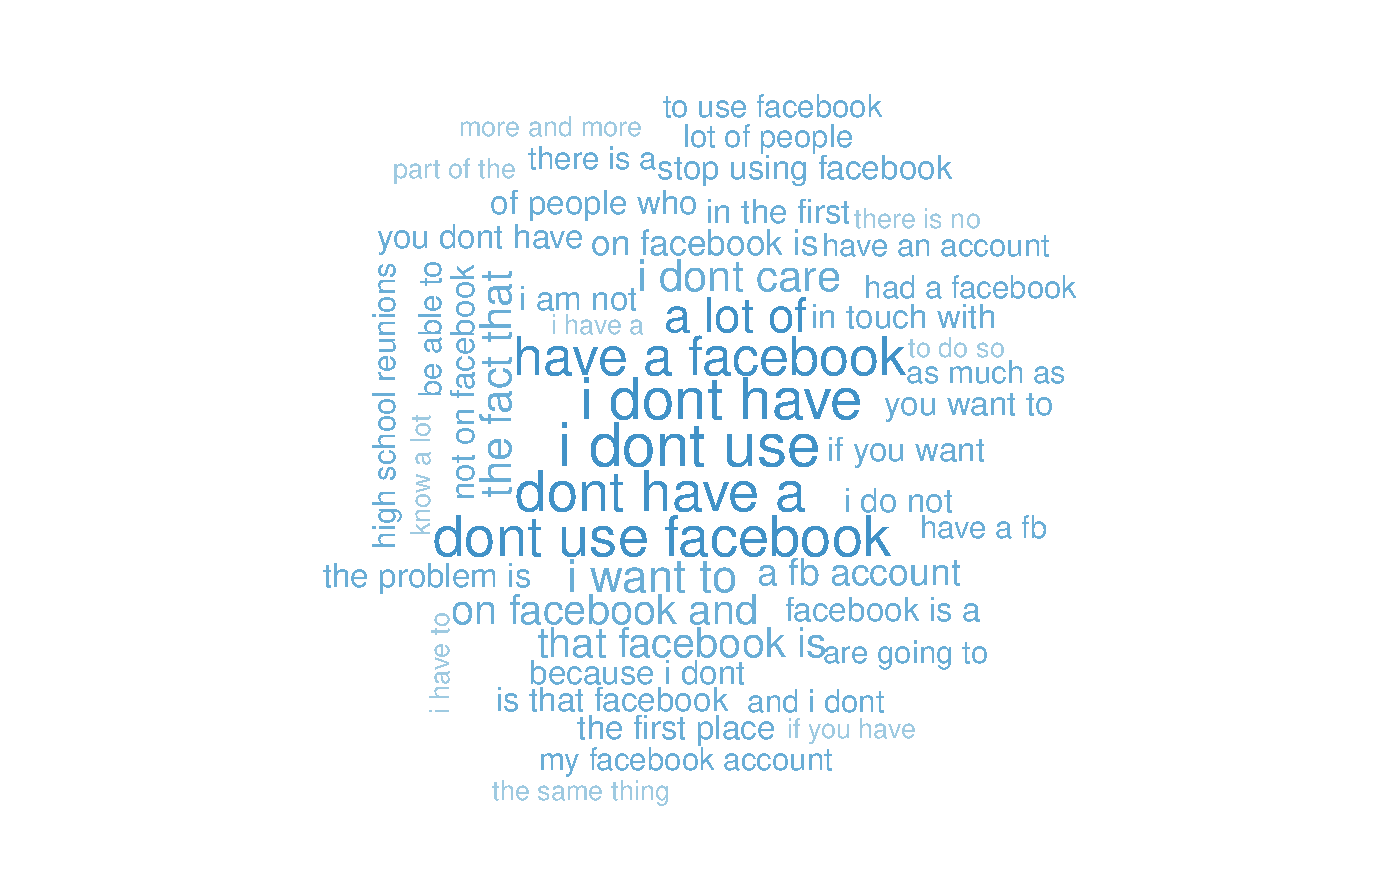
\includegraphics[width=90mm]{figures/fig4.eps}
% }
% \caption{Visualization of 516 \textit{Non-use} comments.}~\label{fig:figure2}
% \end{figure*}


\begin{figure*}
\subfloat[Unigram wordcloud\label{fig:test1}]
  {\includegraphics[width=.3\linewidth, height=4cm]{figures/fig2.png}}\hfill
\subfloat[Bigram wordcloud\label{fig:test2}]
  {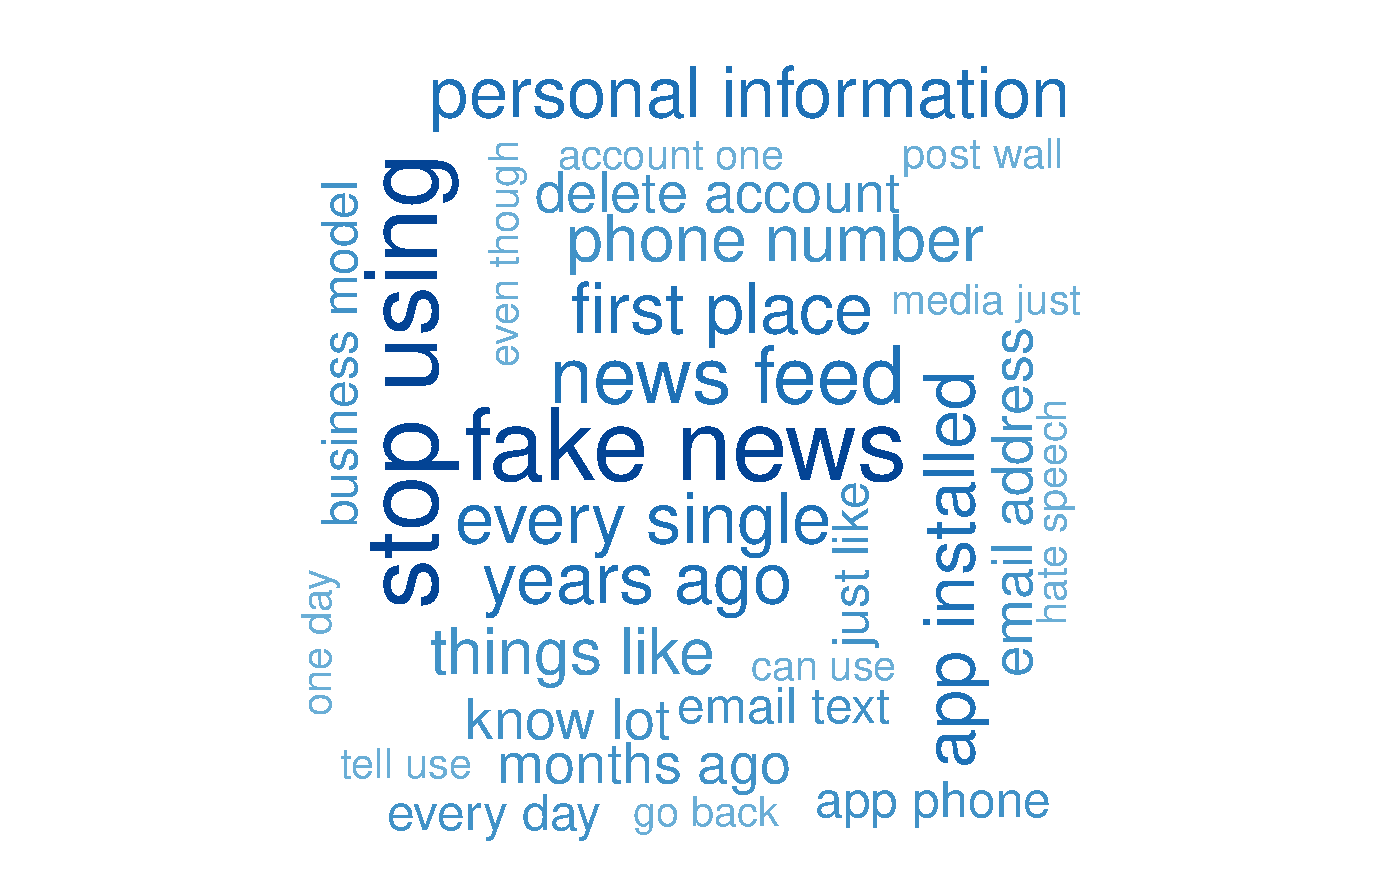
\includegraphics[width=.35\linewidth, height=4cm]{figures/fig3.eps}}\hfill
\subfloat[Trigram wordcloud\label{fig:test3}]
  {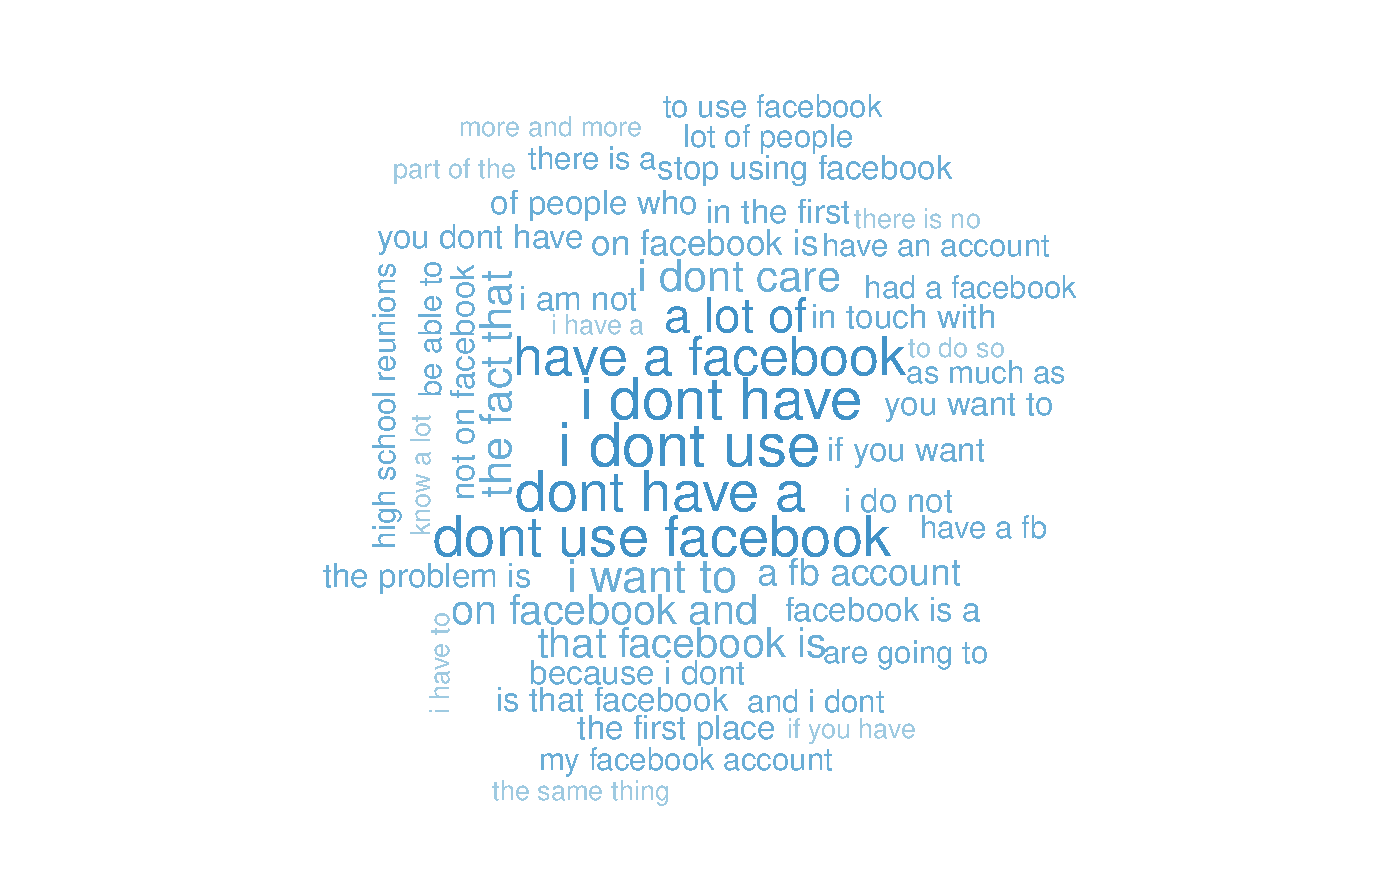
\includegraphics[width=.35\linewidth, height=4cm]{figures/fig4.eps}}
\caption{Visualization of 516 \textit{Non-use} comments.}~\label{fig:figure2}
\end{figure*}




\subsubsection{Topic Modeling}

Our trained LDA model produced 8 topics. Each topic is associated with a weight-distributed set of words. For each weight $w_i$, the weights are normalized such that, $\sum_{i=1}^n w_i=1$. Table ~\ref{tab:table3} lists each topic associated with the word distribution and few selected highly representative words from that distribution those the authors found a match while coding the comments.


\begin{table*}[ht]

\centering
\begin{tabular}{p{0.1\linewidth}|p{0.70\linewidth}|p{0.15\linewidth}}
\hline
\head{Topic \#} & \head{Word Distribution} & \head{Representative Words}\\
\hline
1       & 0.008*"app" + 0.005*"company" + 0.004*"reason"+ 0.004*"feed" + 0.004*"speech" + 0.004*"apps" + 0.004*"data" + 0.004*"privacy" + 0.004*"hate" + 0.004*"always" & hate,privacy\\\hline
2 & 0.012*"social" + 0.008*"stop" + 0.007*"news" + 0.006*"privacy" + 0.006*"ads" + 0.005*"device" + 0.005*"friend" + 0.004*"block" + 0.004*"seen" + 0.004*"political" & news,ads,block\\\hline

3 & 0.011*"social" + 0.009*"information" + 0.007*"stuff" + 0.006*"data" + 0.004*"mean" + 0.004*"provide" + 0.004*"source" + 0.004*"private" + 0.004*"government" + 0.004*"looking" & data,private\\\hline

4 & 0.010*"privacy" + 0.007*"email" + 0.006*"private" + 0.006*"service" + 0.006*"ads" + 0.005*"social" + 0.005*"profile" + 0.004*"information" + 0.004*"world" + 0.004*"name" & privacy,information\\\hline

5 & 0.008*"privacy" + 0.007*"union" + 0.007*"social" + 0.005*"data" + 0.005*"stopped" + 0.005*"personal" + 0.004*"access" + 0.004*"code" + 0.004*"dropped" + 0.004*"left" & stopped,left,dropped \\\hline

6 & 0.013*"information" + 0.010*"social" + 0.009*"personal" + 0.007*"data" + 0.004*"play" + 0.004*"upload" + 0.004*"online" + 0.004*"number" + 0.004*"take" + 0.004*"face"  & social,personal\\\hline

7 & 0.011*"news" + 0.006*"deleted" + 0.005*"tag" + 0.005*"information" + 0.005*"articles" + 0.004*"fake" + 0.004*"business" + 0.004*"stop" + 0.004*"privacy" + 0.004*"free" & deleted,fake,stop\\\hline

8 & 0.008*"social" + 0.007*"data" + 0.007*"news" + 0.005*"money" + 0.005*"might" + 0.004*"problem" + 0.004*"us" + 0.004*"making" + 0.004*"information" + 0.004*"last"  & money,problem\\
\hline
\end{tabular}
\caption{LDA topic modeling on the dataset.}
    \label{tab:table3}
\end{table*}

To confirm the results obtained from LDA model, the topics found from Non-negative Matrix Factorization (NMF) were compared. Table ~\ref{tab:table4} summarizes the top 5 topic words of each topic (Highlighted are the most intereseting and relevant topic words.)


\newcommand{\head}[1]{\textnormal{\textbf{#1}}}

\begin{table}[!ht]
% let LaTeX figure out optimal amount of intercolumn whitespace:
\setlength\tabcolsep{0pt} 

\begin{tabular*}{\columnwidth}{@{\extracolsep{\fill}}c*{3}{T{1.8}}cT{1.8}}  
\toprule
\head{Topic \#} & \head{Topic Words} \\
\midrule
\textbf{1}              & \textbf{social} networking network face email &    \\                    
   \textbf{2} & \textbf{news} \textbf{fake} feed articles trump & \\
   \textbf{3} & \textbf{friend} \textbf{info} word profile mean & \\
   \textbf{4} & \textbf{privacy} information \textbf{private} \textbf{personal} public & \\
   \textbf{5} & \textbf{data} business personal good fact & \\
   \textbf{6} & app installed \textbf{ads} guess android & \\
   \textbf{7} & accounts \textbf{stopped} \textbf{hell} play platform  & \\
   \textbf{8} & \textbf{shit} \textbf{hate} \textbf{share} service public & \\
  \hline
\bottomrule 
\end{tabular*}
\caption{NMF topic modeling on the dataset.}
    \label{tab:table4}
\end{table}

\subsubsection{Sentiment Analysis}

Initially we performed sentiment analysis with VADER tool on our overall set of 516 \textit{Non-use} comments. Then we looked into each of the eight themes to see how the user sentiment compares according to comments belonging to each theme. The VADER tool returns four different measures of sentiment: \textit{pos}, \textit{neg}, \textit{neu} and \textit{compund score}. The compound score can be found by summing the valence scores of each word in the lexicon, adjusted according to the rules. Then it is normalized between -1 to 1, where -1 being extreme negative and +1 being extreme positive. Typically the threshold adopted by researchers ~\cite{hutto2014vader} is: \textit{compound score} >= 0.5 is positive; \textit{compound score} <=-0.5 is negative and anything between -0.5 and 0.5 is neutral. Values of \textit{pos}, \textit{neg} and \textit{neu} can be used instead if multidimensional sentiment analysis of a sentence is desired, where they indicate the percentage of the text that fell into those sentiment categories. In Figure ~\ref{fig:figure6}, we show the box plots of compound sentiment scores for 8 themes as well as the overall set of comments side by side.  


\begin{figure}[t!]
  \centering
  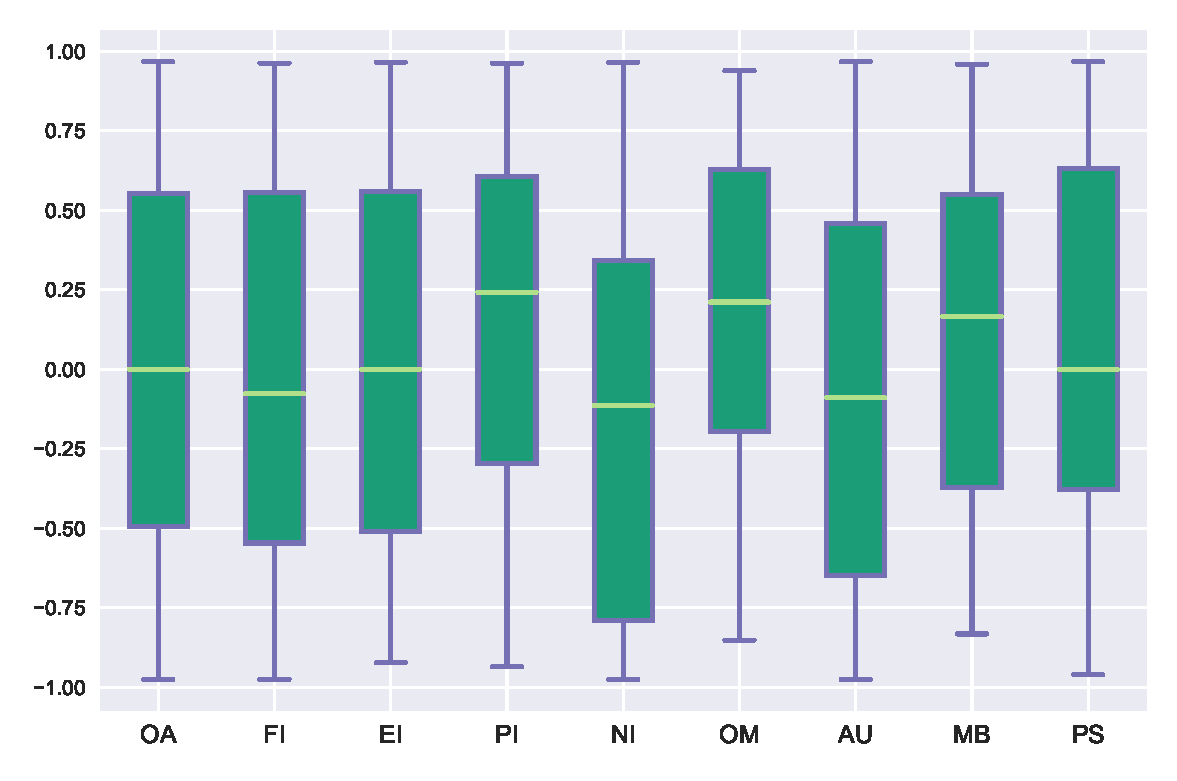
\includegraphics[width=1.0\columnwidth]{figures/fig6.eps}
  \caption{Box plots of compound sentiment scores of each theme using VADER tool. (OA = Overall, FI = Facebook Functionality, EI= Influence of External Factors, PI = Personal Preferences, NI = Negative Perceptions of Facebook, OM = Non-Facebook Media Use, AU = Audience, MB = Modified Behavior, PS = Privacy \& Security)}~\label{fig:figure6}
\end{figure}

For our analysis, we categorize the sentiment associate with the compound score as: $compound score >= 0.5$ is extremely positive; $compound score <-0.5$ is extremely negative, $ 0<=compound score<0.5$ is positive and $-0.5<=compound score<0$ is negative. We calculate the percentage negative per theme as: $$\frac{\text{number of extreme negatives + number of negatives}}{\text{total number of comments belonging to that theme}}$$

The results are reported in Table ~\ref{tab:table5}.

% \newcommand{\head}[1]{\textnormal{\textbf{#1}}}

% \begin{table}[!ht]
% % let LaTeX figure out optimal amount of intercolumn whitespace:
% \setlength\tabcolsep{0pt} 

% \begin{tabular*}{\columnwidth}{@{\extracolsep{\fill}}c*{3}{T{1.8}}cT{1.8}}  
% \toprule
% \head{Theme} & \head{\# Extreme Pos} & \head{\# Pos} & \head{\# Extreme Neg} & \head{\# Neg} & \head{\% Neg}\\
% \midrule
% \textbf{FI}              & 66     & 53 & 59 & 67 & 51.42\%\\                    
%   \textbf{EI} & 16      & 17 & 9 & 16 & 43.10\% \\
%   \textbf{PI} & 33      & 29 & 23 & 11 & 35.41\%\\
%   \textbf{OM} & 10      & 8 & 5 & 4 & 33.33\%\\
%   \textbf{NI} & 13      & 21 & 11 & 31 & 55.26\%\\
%   \textbf{AU} & 17      & 14 & 16 & 20 & 53.73\%\\
%   \textbf{PS} & 58      & 38 & 39 & 33 & 42.85\%\\
%   \textbf{MB} & 8      & 4 & 7 & 3 & 45.45\%\\
%   \hline
% \bottomrule 
% \end{tabular*}
% \caption{Sentiment distribution for 8 themes using VADER method. (FI = Facebook Functionality, EI= Influence of External Factors, PI = Personal Preferences, NI = Negative Perceptions of Facebook, OM = Non-Facebook Media Use, AU = Audience, MB = Modified Behavior, PS = Privacy \& Security)}
%     \label{tab:table5}
% \end{table}


\begin{table}[t!]

\centering
\begin{tabular}{p{0.1\linewidth}|p{0.18\linewidth}|p{0.1\linewidth}|p{0.18\linewidth}|p{0.1\linewidth}|p{0.1\linewidth}}
\hline
\head{Theme} & \head{\# Extreme Pos.} & \head{\# Pos.} & \head{\# Extreme Neg.} & \head{\# Neg.} & \head{\% Neg.}\\
\midrule
\textbf{OA}              & 140     & 135 & 127 & 113 & 46.51\%\\
\textbf{FI}              & 66     & 53 & 67 & 59 & 51.42\%\\                    
  \textbf{EI} & 16      & 17 & 16 & 9 & 43.10\% \\
  \textbf{PI} & 33      & 29 & 11 & 23 & 35.41\%\\
  \textbf{OM} & 10      & 8 & 4 & 5 & 33.33\%\\
  \textbf{NI} & 13      & 21 & 31 & 11 & 55.26\%\\
  \textbf{AU} & 17      & 14 & 20 & 16 & 53.73\%\\
  \textbf{PS} & 58      & 38 & 33 & 39 & 42.85\%\\
  \textbf{MB} & 8      & 4 & 3 & 5 & 45.45\%\\
  \hline
\bottomrule 
\end{tabular}
\caption{Sentiment distribution for 8 themes using VADER method. (OA = Overall, FI = Facebook Functionality, EI = Influence of External Factors, PI = Personal Preferences, NI = Negative Perceptions of Facebook, OM = Non-Facebook Media Use, AU = Audience, MB = Modified Behavior, PS = Privacy \& Security)}
    \label{tab:table5}
\end{table}

% Finally, our trained logistic regression model that was trained on Kaggle data\footnote{\url{https://inclass.kaggle.com/c/si650winter11}} achieved precision, recall and f1-score of 0.98, 0.98 and 0.98 respectively. When applied on unseen comments from our dataset, the classifier results are reported in Table ~\ref{tab:table5}

% \newcommand{\head}[1]{\textnormal{\textbf{#1}}}

% \begin{table}[!ht]
% % let LaTeX figure out optimal amount of intercolumn whitespace:
% \setlength\tabcolsep{0pt} 

% \begin{tabular*}{\columnwidth}{@{\extracolsep{\fill}}c*{3}{T{1.8}}cT{1.8}}  
% \toprule
% \head{Theme} & \head{\#Pos} & \head{\#Neg} & \head{\% Neg}\\
% \midrule
% \textbf{Facebook Functionality}              & 80     & 165 & 67.34\\                    
%   \textbf{Influence of External Factors} & 29      & 29 & 50.00\\
%   \textbf{Personal Preferences} & 25      & 71 & 73.95\\
%   \textbf{Negative Perceptions of Facebook} & 24      & 52 & 68.4\\
%   \textbf{Non-Facebook Media Use} & 4      & 23 & 85.18\\
%   \textbf{Audience} & 20      & 47 & 70.14\\
%   \textbf{Modified Behavior} & 7      & 15 & 68.18\\
%   \textbf{Privacy \& Security} & 62      & 106 & 63.09\\
%   \hline
% \bottomrule 
% \end{tabular*}
% \caption{Sentiment distribution for 8 themes using Logistic Regression method.}
%     \label{tab:table5}
% \end{table}



%% !TEX root=template.tex
\section{Discussion}
\label{sec:discussion}
%Ultimately, we could find some common traits between our users. Facebook's ease and convenience of connecting people is a commonly acknowledged trait between our users, which we expected since this falls in line with why Facebook is such a popular site, to begin with. 7 out of 8 users also said their frequency of posts from their account had decreased over time since they created their accounts. This also falls in line with other literature about Facebook usage since it is commonly observed that original posting has decreased on Facebook in recent years. With 3 users mentioning that they are currently thinking of leaving the site, there is a noticeable trend of users thinking of abandoning the site. Our participants mentioned that they wouldn't leave the site due to the connections that are maintained on Facebook, and the fear of losing contact with some of these friends or family members. 
%There were also quite a few outliers or special insights that only one participant may have mentioned, but are still important factors or insights to consider. P8 mentioned specifically that the participant did not like the fact that the parents are on Facebook. P7 had multiple Facebook accounts, and the most out of any of our participants with 3 Facebook, 2 Twitter, and 5 Reddit accounts. P6 showed strong dissatisfaction about the Facebook account reactivating after 7 days, whereas earlier it would stay deactivated unless you logged back in. 


% !TEX root=nonusecomments.tex
\section{Implications}
\label{sec:implications}
The implications of the findings are manifold: from the perspective of researchers, users, service providers, and system designers \cite{baumer2015importance}. A common psychology in practice is people go with the trend or they tend to follow the crowd ~\cite{gilbert2009blogs}. So from a user's point of view, when other blog readers of Slashdot see such negative emotions associated with Facebook (or any other social media in general), they tend to get biased as well. This is mainly because since the Slashdot and Schneier's blog users are presumably technology geeks, their comments or reviews carry higher weight than usual. These people are early adopters and their knowledge stems from deeper understanding of technology. So if they are expressing \emph{NS} and promoting \textit{Non-use}, decision making of non-experts in terms of social media usage is negatively affected as well. Our \textit{RQ1} results shed light on this. 


Our \textit{RQ2} results have implications on the way future systems could be designed and existing systems could be evaluated. For example, an independent researcher or system designer wants to evaluate any existing blog or forum for user satisfaction level. With help of the techniques adopted in answering \textit{RQ1} and \textit{RQ2} or a similar but modified approach, a sentiment classifier can be built and user sentiment for that particular blog/forum can be assessed. This way product business related blog/forums could be benefited too because such blogs contain high volume unprompted reviews from users (e.g., Yelp, Amazon) and their target audience are the buyers. Our approach will enable them to understand user behavior or sentiment and adjust their business model accordingly. This knowledge can also be applied for developing a new media for communication too since traditional usability study of newly developed system is time consuming. We believe the most important implication for our \textit{RQ2} results is practical. For instance, a Facebook system analyst can go through the finding of this work to get a top level idea of what is affecting user engagement and ways to fix them. Leveraging the findings of the 10 influential factors and sentiment associated with them, it can be deduced that Facebook needs to improve their system architecture and enhance privacy and security measures. The findings offer implications for system designers and HCI researchers too. Our findings suggest that, for both dataset users are mostly concerned with privacy and security issues while user experience and personal preference play a secondary role. It has to be understood that technology use is more a cultural phenomenon \cite{satchell2009beyond} so the study of \emph{Non-use} and use has to be considered from that perspective. The findings do not necessarily point to a radical design change or complete disposal rather it suggests naturalistic responses on what are design flaws and what changes can incorporate more users. Many users suggested how staying away from social media for a while helped them to better balance their social life. So Facebook designers can consider \emph{Non-use} positively and possibly facilitate it by allowing the users to take temporary breaks, strategies to balance user interaction with social media \cite{schoenebeck2014giving} and enabling more self-inhibiting options without `undesigning' it \cite{pierce2012undesigning}. As Baumer and Silverman \cite{baumer2011implication} argued, designers should consider the implication when not to design \cite{dourish2006implications} but this does not promote rejection of technology. One Slashdotter addressed this issue in his comment:
\begin{quote}
         \textit{You never really leave Facebook. I thought I had deleted my account but signed back in a month later and it was still there. All my friends still present. Even the pictures and comments I had deleted individually were still there.}
    \end{quote}
Exact similar sentiment regarding Facebook account deactivation was found by another user of Schneier on Security: \textit{"My question is if I delete my Facebook is it ever really gone? I would love to get rid of it but my friends would think I'm no longer friends with them and take it to heart which I think is stupid. I've heard of stories of deleting a Facebook then coming back years later and everything is just how you left it."} It is evident that Facebook currently disregard the ongoing movement in terms of \emph{Non-use}. Our findings have critical implications for UI designers of Facebook in this regard. Incorporating ideas from non-users guarantee an engaged user-base and can bring positive sociotechnical changes \cite{baumer2013limiting}. On the other hand, if they do not facilitate users who willingly decide to withdraw or recess, the looming \emph{NS} of Facebook users can be menacing for them. Today the non-users may not be an overwhelming majority but their perspective should be valued and dealt with \cite{wyatt2003non, satchell2009beyond}, especially if they are tech-savvy users. A more deeper analysis will reveal other system pitfalls and ways to overcome them. This is significant for users and developers alike because it will enable them to create an all inclusive environment that is devoid of the factors discovered in our findings.

% !TEX root=nonuseinterviews.tex
\section{Limitations}
\label{sec:limitations}
Our study had a few limitation, due to the qualitative nature of the study and personal interviews the demographics were skewed mostly towards students. We tried to keep our focus on interviewing participants who expressed reduction in their Facebook usage or do not have a Facebook account out of which 5 participants who did not have a Facebook account. Though this number seems to be low however, all of them had different reasons for not having a Facebook account, as discussed in the section~\ref{sec:findings}, which is quite astonishing. We want to validate the reasons by extending the study to study quantitative data as one of the future directions, however when we talk about user experience aiming at insightful discussions, qualitative methods are the best to follow. While users have expressed concerns about the data usage policies of Facebook however, lack of proper communication and implication of such policies indicates that privacy is not the major deciding factor in determining personal usage of the social media website, which though surprising is understandable. This is again proved by those who are migrating to other social media websites, thus they are concerned on specifically Facebook rather than the data usage. Those who choose not to have any social presence choose one-one communication.


%% !TEX root=nonusecomments.tex
\section{Future Work}
\label{sec:futurework}
Our findings engender interesting potential research questions: Do we get similar user sentiments towards other non-Facebook privacy sensitive media? Does incorporating more data and application of machine learning based text classification approach guarantee successful prediction? For our future work we want to explore other sources where users discuss their Facebook user experience to get a comprehensive understanding. In particular, this will be interesting to analyze if the underlying factors found in this study from expert users are consistent with other data sources consisting of general audience. This however, is not feasible to answer in a single paper, since everyday more and more such platforms are emerging and also analysis of a particular site provides answers to problems of specific audience. Design and implementation of a text classifier, which will significantly reduce the human effort and automate the process, is also left as future work. Unsupervised machine learning based approaches, such as clustering, topic modeling, opinion mining can be applied to detect inherent motives automatically. Also, we would like to extend the knowledge gathered from this study to address more generic agenda, such as overall social media (not only Facebook) sentiment mining. We want to use more hand annotated data for future analysis as it will not only increase the accuracy but also help getting our domain specific sentiment.

% !TEX root=foo.tex
\section{Conclusion}
\label{sec:conclusion}
This paper aims to address an under-researched issue in the field of user interaction with technology, namely, social media \textit{Non-use}. We believe this is imperative to understand the mindset of tech-savvy non-participants and the factors that play a pivotal role in this regard. We collected user generated comments from a technology blog called Slashdot and through qualitative coding got significant responses related to \textit{Non-use}. Further analysis unveiled several user dissatisfaction related to Facebook, for example, flaws in Facebook architecture, privacy and security concerns, personal issues etc. These results were bolstered by NLP based automated analysis and it turned out that the results of both approaches are consistent. Our findings have manifold implications for non-expert users, system designers, business analysts in designing and evaluating a reliable, fail-safe system. Besides, our work invokes several interesting questions, for example, Does availability of more data enable us to perform temporal (time-series) sentiment analysis on non-participants? How do the same techniques apply to other sources of data comprised of diverse population (layman and tech-savvy)? 

% !TEX root=nonuseinterviews.tex
\begin{acks}
Anonymous for blind review.
\end{acks}

% Bibliography
\bibliographystyle{ACM-Reference-Format}
\bibliography{references_nonuseinterviews}

%%\section{Appendix}
%\label{sec:Appendix}
\begin{appendices}
%\appendixname{Appendix}
%\appendix
\textbf{A. SCREENING QUESTIONNAIRE}
\\
Thank you for your interest in participating in our study on Online Communication Practices.   Please fill out this brief 1-minute questionnaire regarding yourself and your online communication choices. We will utilize your answers to determine if you are eligible to participate in the study. If you qualify, we will contact you via email for a 30-45 minute in-person/ video conference/ telephone interview for which you will receive $10 cash/$10 Amazon gift certificate as a token of our appreciation for your participation. If you do not qualify for participation, your responses will be safely discarded. 
\begin{enumerate}
\item What is your Year of Birth?
\item Which Gender do you identify with the most?
\begin{itemize}
\item Female
\item Male
\item Other- Please Specify:
\item Do not wish to specify
\end{itemize}
\item Are you affiliated with ANONYMOUS University?
\begin{itemize}
\item Yes
\item No
\end{itemize}
\item (If affiliated with ANONYMOUS University) What is your affiliation with ANONYMOUS University? (Check all that apply.)
\begin{itemize}
\item Undergraduate Student
\item Graduate Student
\item Faculty
\item Staff
\item Retired
\item Other - Please Specify:
\end{itemize}
\item How long have you been living in the US?
\begin{itemize}
\item Less than a year
\item 1 year
\item 2 years
\item 3 years
\item 4 years
\item 5 years
\item 6 years
\item 7 years
\item 8 years
\item 9 years
\item 10 years
\item 11 years
\item 12 years
\item 13 years
\item 14 years
\item 15 years
\item 16 years
\item 17 years
\item 18 years
\item 19 years
\item 20 years
\item More than 20 years
\end{itemize}
\item Do you have a Facebook account?
\begin{itemize}
\item Yes
\item No
\end{itemize}
\item (If Yes to Facebook account) What do you use Facebook for? (Check all that apply.)
\begin{itemize}
\item Posting Status Updates, Pictures, Videos, etc.
\item Reading the News Feed.
\item Commenting on Others' Posts.
\item Liking Others' Posts.
\item Messaging Facebook Friends.
\item Other - Please Specify:
\end{itemize}

\item (If Yes to Facebook account) Compared to a year ago, how often do you post on Facebook?
\begin{itemize}
\item More often than a year ago.
\item About the same amount as a year ago.
\item Less often than a year ago.
\end{itemize}
\item (If Yes to Facebook account) How would you characterize your use of Facebook?
\begin{itemize}
\item I write/post/produce more than I read/click/consume.
\item I read/click/consume more than I write/post/produce.
\item I write/post/produce roughly the same amount as I read/click/consume.
\item Please elaborate:
\end{itemize}
\item If you qualify for the study, which email address should we use to contact you for scheduling an in-person/ video conference/ telephone interview?
\item (If not affiliated with ANONYMOUS University) How would you prefer to be interviewed?
\begin{itemize}
\item Video Conference
\item Telephone Interview
\end{itemize}
\end{enumerate}
\textbf{B. SEMI-STRUCTURED INTERVIEW QUESTIONS}
\textbf{\textit{Social media accounts}}
\begin{enumerate}
\item Do you currently have a Facebook account you actively use?
\item What other social media platforms do you use?
\item Do you use your Facebook account to login to other services on the Internet? Why or why not?
\end{enumerate}
\textbf{\textit{If participant does not have a Facebook account}}
\begin{enumerate}
\item Did you ever have a Facebook account?
\item If Yes, why did you choose to get rid of the Facebook account?
\item If No, why did you choose not to create a Facebook account?
\item If No, is there anything that would prompt you to create a Facebook account in future?
\item If No, what do you believe you are gaining or missing by not having a Facebook account?
\end{enumerate}
\textbf{\textit{If participant has a Facebook Account}}
\begin{enumerate}
\item What prompted you to create a Facebook account?
\item How long have you had a Facebook account?
\item Why do you use Facebook?
\item What aspects of using Facebook do you like?
\item What aspects of using Facebook do you dislike?
\item Which features of Facebook do you typically use (i.e., chat, groups, events, etc.)? Why?
\item How often do you post on Facebook?
\item What do you post?
\item How has your posting on Facebook changed over time?
\item If reduced or increased, was the change abrupt or gradual? Why?
\item If reduced or increased, how is it related to changes in Facebook?
\item If reduced or increased, how is it related to changes in your own life and views?
\item In what ways is Facebook satisfying to use?
\item In what ways is Facebook dissatisfying to use?
\item In what ways is Facebook useful or productive?
\item In what ways is Facebook not useful or unproductive?
\item What role does Facebook play in your life?
\end{enumerate}
\textbf{\textit{Facebook Behavior}}
\begin{enumerate}
\item What do you think people think of you based on your Facebook profile?
\item How do you decide what you post on Facebook?
\item How do you manage how Facebook makes you look to others?
\item How do you decide what to include or leave out in your posts?
\item Have you ever posted anything that you later edited or deleted?
\item If yes, why did you edit or delete it?
\item Have you ever regretted a post after you made it? If yes, why? What did you do about the regret?
\item In what ways are you a producer of information on Facebook?
\item In what ways are you a consumer of information on Facebook?
\item Which of the two modes (producer and consumer) is your predominant or preferred way of using Facebook? Why? 
\end{enumerate}
\textbf{\textit{Facebook Privacy}}
\begin{enumerate}
\item In what ways is your use of Facebook “public”?
\item In what ways is your use of Facebook “private” or restricted?
\item What are your privacy settings on Facebook? (public, friends only, only me, others)
\item Why did you choose these settings?
\item When do you change your privacy settings? How often?
\item Do you restrict yourself from being seen on Facebook? If yes, in what way?
\item Have you ever unfriended or blocked your friends on Facebook? If yes, why?
\item What do you believe Facebook uses your data for?
\item What do you think about Facebook’s policies regarding the use of your Facebook data?
\item What do you feel about sharing data and information on Facebook?
\end{enumerate}
\textbf{\textit{Abandoning Facebook/Returning to Facebook}}
\begin{enumerate}
\item Do you ever feel like leaving Facebook entirely (deleting your account)? If yes, why? If no, what about curtailing or restricting your Facebook use? If yes, why and in what ways?
\item If you delete/deactivate your Facebook account, which other systems would you switch to? Why?
\item Do you know anyone who has deactivated their Facebook account or stopped or reduced use of Facebook? If yes, why did they do so?
\item Have you ever deactivated your Facebook account? If yes, why? Did you reactivated it later? If yes, why?
\end{enumerate}
\textbf{\textit{Demographic Questions}}
\begin{enumerate}
\item Where did you grow up?
\item What do you do?
\item If you study, what is your major?
\end{enumerate}
\textbf{\textit{Ending Question}}
\begin{enumerate}
\item Is there anything else regarding your Facebook usage that you would like to share with us?
\end{enumerate}
\end{appendices}
\end{document}